% 4% \documentclass[sigconf,authordraft]{acmart}
% \documentclass[sigconf]{acmart}
% \documentclass[sigconf, screen, review, anonymous]{acmart}
\documentclass[sigconf, screen, review]{acmart}
%%


% \usepackage{tikz}
% \usepackage{arydshln} % for dashed lines in tables
\usepackage[table]{xcolor}
\usepackage{multirow}
\usepackage{graphicx}
\usepackage{booktabs}
\usepackage{siunitx}
\usepackage{subfigure} 
\usepackage{adjustbox}
% \usepackage{makecell, }
\usepackage{makecell}
\usepackage{multirow}
\usepackage{booktabs}
\usepackage{pifont}
\usepackage{subcaption}
% \usepackage{adjustbox}
\usepackage{lipsum} % foor dummy text
\usepackage{xcolor}  % 确保导入了这个包


\usepackage{rotating} % for sidewaystable

% \definecolor{fuchsia}{RGB}{180, 30, 150}
\definecolor{fuchsia}{HTML}{FF0B55}

% FF0B55

\makeatletter
\def\@authornotemark{} % 去除标记符号
\makeatother

% \usepackage[capitalise,nameinlink]{cleveref}
\usepackage[capitalise]{cleveref}  % 去掉 nameinlink
\settopmatter{printacmref=false}
\renewcommand\footnotetextcopyrightpermission[1]{}

% 定义 Figure 显示为带大写首字母的 Figure
\crefname{figure}{Figure}{Figures}
\Crefname{figure}{Figure}{Figures}
\crefname{table}{Table}{Tables}
\Crefname{table}{Table}{Tables}
% \makeatletter
% \crefformat{figure}{Figure~\hyperref[#1]{\ref*{#1}}}
% \Crefformat{figure}{Figure~\hyperref[#1]{\ref*{#1}}}
% \makeatother
% \renewcommand{\thefootnote}{\fnsymbol{footnote}}
% \footnotetext[1]{Equal contribution.}
% \footnotetext[2]{Corresponding author.}


\usepackage{CJKutf8} % 中文支持

% \newcommand{\bobo}[1]{{\color{cyan}Bobo: #1}}
\newcommand{\bobo}[1]{%
  \begin{CJK}{UTF8}{gbsn} % 开启中文环境
  {\color{cyan}Bobo: #1}%
  \end{CJK}%
}


% 全局设置:数值对齐,保留一位小数(除相关系数保留四位)
\sisetup{
  detect-mode,
  mode=text,
  group-digits = false,
  round-mode     = figures,
  round-precision= 2,
  table-number-alignment = center,
  table-figures-integer = 1,
  table-figures-decimal = 1,
  detect-all,
  output-decimal-marker = {.}
}




\AtBeginDocument{%
  \providecommand\BibTeX{{%
    Bib\TeX}}}

\begin{document}

%%
\title{FormFactory: An Interactive Benchmarking Suite for Multimodal Form-Filling Agents}

\author{Bobo Li$^{\#1}$, Yuheng Wang$^{\#2}$, Hao Fei$^{*1}$, Juncheng Li$^3$, Wei Ji$^4$, Mong-Li Lee$^1$, Wynne Hsu$^1$}
\affiliation{
  \institution{$^1$National University of Singapore \quad
               $^2$Wuhan University \quad
               $^3$Zhejiang University \quad
               $^4$Nanjing University}
               \city{}
\city{\{libobo, haofei37, dcsleeml, dcshsuw\}@nus.edu.sg, yuhengwang@whu.edu.cn, junchengli@zju.edu.cn, weiji@nju.edu.cn}
\country{Project Page: 
% \textcolor{violet}{X}
% \textcolor{violet}o{\url{https://formfactory-ai.github.io}}}
\href{https://formfactory-ai.github.io}{\textcolor{fuchsia}{\textbf{https://formfactory-ai.github.io}}}}
% \url{https://formfactory-ai.github.io}}
}
% \thank
\email{}
\renewcommand{\shortauthors}{Li et al.}


% \authornote{Hao Fei is the corresponding author, $^\#$ Equal Contribution.}
\authornote{Hao Fei is the corresponding author. $^\#$ indicates equal contribution.}

% \author{Bobo Li$^\#^1$, Yuheng Wang$^\#^2$, Hao Fei$^1$, Juncheng Li$^3$, Wei Ji$^4$, Mong-Li Lee$^1$, Wynne Hsu$^1$}
% \affiliation{%
%   \institution{
%   National University of Singapore$^1$, Wuhan University$^2$, Zhejiang University$^3$, Nanjing University$^4$
%   }
%   \city{}
%   \country{}
%   }
% \email{{libobo, haofei37, dcsleeml, dcshsuw}@nus.edu.sg, yuhengwang@whu.edu.cn, junchengli@zju.edu.cn, weiji@nju.edu.cn}

\begin{abstract}
Online form filling is a common yet labor-intensive task involving extensive keyboard and mouse interactions. 
Despite the long-standing vision of automating this process with “one click,” existing tools remain largely rule-based and lack generalizable, generative capabilities.
Recent advances in Multimodal Large Language Models (MLLMs) have enabled promising agents for GUI-related tasks in general-purpose scenarios.
However, they struggle with the unique challenges of form filling, such as flexible layouts and the difficulty of aligning textual instructions with on-screen fields.
To bridge this gap, we formally define the form-filling task and propose FormFactory—an interactive benchmarking suite comprising a web-based interface, backend evaluation module, and carefully constructed dataset. 
Our benchmark covers diverse real-world scenarios, incorporates various field formats, and simulates high-fidelity form interactions.
We conduct a comprehensive evaluation of state-of-the-art MLLMs and observe that no model surpasses 5\% accuracy, underscoring the inherent difficulty of the task.
These findings also reveal significant limitations in current models’ visual layout reasoning and field-value alignment abilities.
We hope our benchmark can serve as a stepping stone for further research into robust, practical form-filling agents. 
% The FormFactory benchmark is released under the MIT License and is publicly available at \url{https://formfactory-ai.github.io}.

% Project page: \href{https://formfactory-ai.github.io}{https://formfactory-ai.github.io}.

% Online form filling is a complex task that involves extensive keyboard and mouse operations, while the vision of automatically completing forms with "one click" remains highly desirable. 
% Existing assistive tools are primarily rule-based and struggle with generative capabilities, making it difficult to effectively reduce the burden on users during the form filling process. 
% Multimodal Large Language Model (MLLM)-based GUI agents present a promising direction for this task; however, current research in GUI agents is primarily focused on general domains and lacks the capability to handle form filling tasks.
% To address this challenge, we pioneer the formalization of the form filling task and explore viable pathways to tackle it. 
% Specifically, we analyze the real-world scenarios in which form filling occurs and develop an interactive benchmark tool suite, named FormFactory, which includes a web interface, a backend evaluation module, and a dedicated dataset.
% Our tool suite covers multiple realistic scenarios, contains vairous format of fields, and provides a high-fidelity simulation of real-world forms.
% We then conduct a comprehensive evaluation of several state-of-the-art MLLMs on our benchmark, and the suboptimal results highlight the inherent difficulty of the task.
% Finally, we discuss several promising directions to further facilitate automatic form filling and hope our work will provide meaningful contributions to this emerging research area.
% The website of our project is available at \href{https://formfactory-ai.github.io}{https://formfactory-ai.github.io}.
% 
% \hyperlink{https://formfactory-ai.github.io}{https://formfactory-ai.github.io}.

\end{abstract}

%%
%% The code below is generated by the tool at http://dl.acm.org/ccs.cfm.
%% Please copy and paste the code instead of the example below.
%%
\begin{CCSXML}
<ccs2012>
   <concept>
       <concept_id>10002951.10003227.10003251</concept_id>
       <concept_desc>Information systems~Multimedia information systems</concept_desc>
       <concept_significance>500</concept_significance>
       </concept>
   <concept>
       <concept_id>10003120.10003121</concept_id>
       <concept_desc>Human-centered computing~Human computer interaction (HCI)</concept_desc>
       <concept_significance>500</concept_significance>
       </concept>
 </ccs2012>
\end{CCSXML}
\ccsdesc[500]{Information systems~Multimedia information systems}
\ccsdesc[500]{Human-centered computing~Human computer interaction (HCI)}




%%
% \keywords{Do, Not, Us, This, Code, Put, the, Correct, Terms, for,
  % Your, Paper}
\keywords{
Multimodal Large Language Model, 
GUI Agent, 
Form Filling, 
Vision-Language Alignment. 
% Web Automation, 
% Interactive Benchmark, 
% Human-Computer Interaction
}

\maketitle


\section{Introduction}
% \bobo{Intro有些地方逻辑不对,有的不够凝练,有的存在事实性错误(bobo)}

% Filling out online forms has become a common task in daily life, such as when applying for jobs, submitting to conferences or journals, or interacting with enterprise automation systems, as show in the left part of \cref{fig:fig1}.
% In these scenarios, users are required to select suitable options and input corresponding text, aligning their profiles with the form fields for efficient information collection and management.
% Although this design simplifies the management process, it often requires excessive interaction with the form using a mouse and keyboard.
% For example, during job application seasons, users must repeatedly input duplicate information in various website, such as personal profiles, while also customizing specific content to adapt the unique layout of each website.
% Therefore, an ideal solution to automate the form-filling process and replace the manual operation of the keyboard and mouse has long been a sought-after goal.
% \bobo{a description of the dataset and the dataset 

% generation process

% licencing and access

% potential applications

% reproducibility and supplementary materials

% ethical considerations and privacy (if applicable)

% A baseline solution (if applicable)}
Filling out online forms is a common yet tedious task in many scenarios such as job applications, academic submissions, and enterprise workflows, as illustrated in \cref{fig:fig1}.
Although users often already possess the required information—such as personal background, publication details, or leave dates—they must still carefully navigate each interface, locate the correct fields, and manually align their input.
For instance, during job-hunting season, applicants adaptively input the same resume content across a wide range of online job platforms, each with its own layout, field order, required inputs, and interaction logic.
As a result, automating the form-filling process and eliminating low-level keyboard and mouse operations has long been a highly desirable goal.

% \begin{figure}[!t]
% \centering
% \includegraphics[width=0.93\columnwidth]{figs/sample}
% \vspace{-3mm}
% \caption{
% Prompt designed to guide ChatGPT in the task of extracting emotion-cause pairs from dialogue, illustrating the specific instructions, input, and output formats used.
% }
% \label{fig:gpt}
% \end{figure}

\begin{figure*}[t]
    \centering
    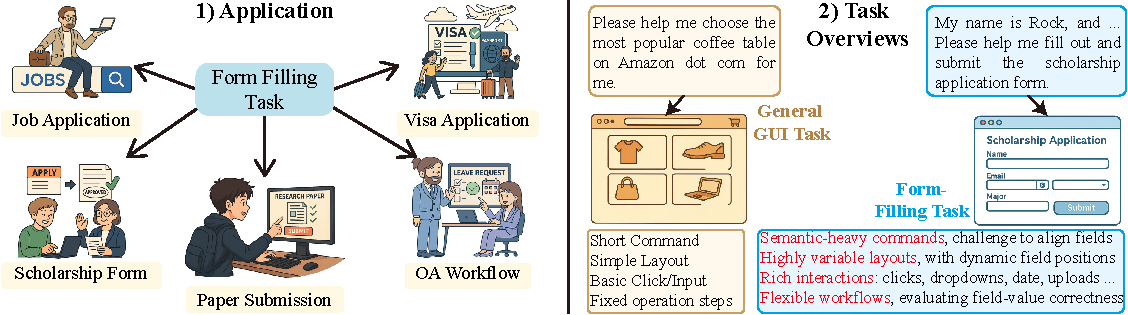
\includegraphics[width=0.93\linewidth]{figs/fig1v1.pdf}
    \caption{Overview of the form-filling task and its challenges. Compared to general GUI tasks, form-filling involves more diverse applications and demands higher semantic understanding, layout flexibility, and interaction complexity.}
    \label{fig:fig1}
\end{figure*}

% To clarify, we define the automate scenario of requirement as follows: In the form-filling context, we have a document and an interactive online form.
% The document contains preliminary information, such as a resume for job applications or a leave request with details like time and location.
% The online form consists of various fields and values, such as name, birth date, job title, and educational background, with different formats for input, including text fields, dropdown lists, checkboxes, date pickers, and file uploads.
% Given the document and the form, the model must understand both the document and the form structure.
% It should then output a sequence of click and mouse operations to guide the user through the form-filling process based on the information in the document, ultimately submitting the form.

% While some basic solutions exist—such as Chrome’s ability to auto-fill addresses —these rule-based methods are limited to fixed personal information and often fail in more dynamic scenarios with diverse or irregular field structures.
While basic solutions like Chrome’s address autofill exist, such rule-based methods are confined to static fields and often fail in dynamic or irregular form scenarios.
Some platforms offer semi-intelligent features, such as parsing uploaded resumes into structured fields on job application sites.
% To improve user experience, certain platforms have introduced semi-intelligent features.
% For instance, job application website may allow users to upload resumes that are automatically parsed into various fields on the platform.
While helpful, these systems still struggle with accurate field-to-content alignment, particularly when dealing with nuanced distinctions or ambiguous contexts.
For example, internships may be erroneously parsed as full-time employment, distorting the applicant’s profile and demanding manual adjustments.
Accurate parsing remains unreliable even for a single form on a single site, and the diversity of real-world forms only amplifies the challenge. 
Building dedicated parsers for each platform, with its unique input types, HTML structures, and layouts, is prohibitively labor-intensive and ultimately unsustainable.
This raises a natural question: can we build a general-purpose vision agent that completes any form on any website by visually parsing the interface, retrieving relevant information, reasoning over field-value alignment, and executing the full interaction flow?

% This raises a natural question: can we build a general-purpose vision agent that ocompletes any form on any website—by visually parsing the interface, retrieving relevant materials, reasoning about field-value alignment, and executing the full interaction flow?
% This raises a natural question: instead of hardcoding HTML-specific logic, can we develop a general-purpose, vision-based agent that fills out any form—on any website—just like a human? 
% Such an agent would visually observe the screen, retrieve relevant materials (e.g., resumes, submissions, leave requests), reason about the appropriate inputs and their locations, interact with the interface, and complete the submission process end-to-end.


% While form-filling has been some basic solutions for users, such as the ability of Chrome to remember location information and enable one-click input, these rule-based methods are typically limited to personal information entry.
% For most dynamic scenarios, where field names are more diverse or involve additional information, these methods perform poorly.
% Some websites have developed more advanced methods.
% For instance, job application websites offer the option to upload a user’s resume, which is then parsed into specific fields such as educational experience and work history.
% Although this approach incorporates some intelligence, the user experience remains suboptimal, particularly when it comes to field alignment.
% For example, a project experience might be incorrectly placed under the "research" field.

% Furthermore, these methods require reading the HTML source code and developing specific code for each website.
% The source data varies significantly between different systems, such as job search portals, paper submission sites, and enterprise automation systems.
% It is impractical to expect every website to develop its own intelligent parser for aligning fields.
% As a result, there is still a lack of tools capable of alleviating the human burden in form-filling tasks.

% To address this problem, we can draw inspiration from how humans fill out forms. Humans possess visual understanding capabilities that allow us to read web pages, understand the semantics of fields, and fill out forms using information stored in memory or documents, all without needing to read the HTML source code.

% Consequently, we propose using a more intelligent, generalized agent to perform form-filling tasks, mimicking how a human would interact with the screen and click buttons.
% With the emergence of Multimodal Large Language Models (MLLMs)\cite{arlt21icml, jlbb22icml, hlvi23nips, pwqv24corr}, several GUI agents\cite{lzst24iclr, psfp23nips, whca24cvpr, kcsh24acl} have been developed.
% These agents can understand human commands, read screenshots, and output a series of screen operations to execute the user's requests.

% Although these agents have shown performance in various benchmarks~\cite{tswo17icml, craa23nips, jzai24emnlp} across different scenarios, such as app installation, web shopping, and account login, they are not directly applicable to form-filling tasks due to several challenges:

With the rise of MLLMs\cite{arlt21icml, jlbb22icml, hlvi23nips, pwqv24corr}, vision-based GUI agents have become increasingly feasible\cite{lzst24iclr, psfp23nips, whca24cvpr, kcsh24acl}.
These agents can interpret natural language instructions, perceive screen content, and execute sequences of keyboard and mouse operations to fulfill user intents.
While they have demonstrated promising performance on benchmarks for general GUI domain~\cite{tswo17icml, craa23nips, jzai24emnlp}, existing GUI agents fall short in handling form-filling tasks.
The challenges arise from three key differences:
First, form filling requires \textbf{fine-grained semantic alignment} between user-provided content (e.g., resumes) and corresponding on-screen fields. Unlike typical GUI tasks driven by explicit commands (e.g., ``install Chrome''), form filling hinges on accurately matching textual information to varied visual labels.
Second, web forms exhibit \textbf{significant structural variability}, including diverse field types, flexible layouts, and inconsistent naming conventions.
The absence of consistent patterns challenges the agent’s ability to generalize and calls for robust visual reasoning and layout comprehension. 
Table comprehension alone presents a significant challenge \cite{zhao24nips, li25www, zheng24acl} for MLLMs; form filling adds the extra complexity of aligning external content and interacting with UI elements.
Third, form filling entails \textbf{increased interaction complexity}.
Beyond basic clicks and typing, it often involves multi-step operations such as handling drop-downs, date pickers, or multi-checkbox inputs, all requiring precise action planning and interface-state awareness.
Moreover, the \textbf{non-determinism in field-click order} makes golden trajectories ambiguous, complicating supervised learning.
% Additionally, form understanding itself is a complex task, and filling it out further amplifies this challenge.
Collectively, these challenges place greater demands on the model’s visual grounding and semantic alignment capabilities.

% \begin{itemize}
%     \item Increased Action Complexity: Form-filling tasks involve more complex actions, particularly in aligning value areas with field names. This is especially challenging when dealing with mixed typography, such as vertical and horizontal text alignment, which requires sophisticated layout and vision understanding capabilities.

% \item Flexible Evaluation Criteria: Unlike other tasks, form filling is more flexible in terms of evaluation. The order in which fields are filled is not crucial, as long as the final form is correctly completed, it will be considered a correct operation.

% \item Complex Actions: Form-filling may involve actions like selecting dates from a calendar or interacting with drop-down lists, which are distinct from the typical button-click or text-box operations handled by general GUI agents.
% \end{itemize}

% Additionally, form understanding itself is a complex task, and filling it out further amplifies this challenge.

% Second, form filling requires alignment with external knowledge.
% Current GUI agents \cite{xdmt23nips, txob24nips} typically rely on human commands as input, without incorporating external data.
% They complete tasks based solely on understanding commands, such as clicking a browser or searching a keyword.
% In contrast, a form agent must read the provided data and align it with the corresponding fields in the form, performing form filling with semantic understanding.
% Additionally, while GUI agents may require human intervention for tasks such as purchasing products or browsing posts, which demand significant human effort, a form agent can alleviate much of this burden by automating the alignment of information.

Despite the practical importance and complexity of form filling, there is still no dedicated benchmark to support evaluation, let alone any well-developed models.
Existing GUI benchmarks~\cite{jzai24emnlp, craa23nips} primarily target general-purpose tasks such as app navigation or basic web operations.
However, these benchmarks fall short of addressing the specific demands of form filling, such as semantic alignment, flexible layout handling, and interaction complexity, making them unsuitable for this task.
Therefore, a reliable, interactive, and form-filling-specific benchmark is urgently needed to facilitate evaluation and further research in this domain.

% Third, there is a lack of an evaluation framework and datasets for form-filling tasks. Current GUI agents~\cite{jzai24emnlp, craa23nips} generally rely on screenshots to perform tasks, but static evaluations like these cannot fully reflect the agent's performance in real-world applications. While some interactive frameworks~\cite{sywt22nips, szwa24iclr} exist, they primarily focus on mobile platforms and general app operations, not on form filling—a specialized and urgent scenario. Moreover, form-filling tasks differ significantly from general GUI tasks, and without a corresponding dataset or interactive framework, model development and evaluation are hindered. Despite the urgent need for form agents, progress in this area has been slow.

% To address this issue, it is essential to build a benchmark tailored to the form-filling domain, incorporating novel data, a real interactive platform, and new evaluation criteria.

% In this paper, we formally introduce a form agent tool suite, named AgentFactory. Our suite includes:
% 1) A form-agent online interaction platform, featuring 20 types of web pages, such as recruitment websites and OA systems.
% The platform includes both a front-end and back-end, enabling access to model results for evaluation.
% It also allows dynamic modification of fields, deletion of fields, and layout adjustments, helping to improve the generalization across websites.

% 2) A series of datasets for various scenarios, generated through instruction learning.
% The dataset includes original documents, such as resumes, papers, and text, as well as webpage fields, with annotations for each field across different webpages, making it suitable for benchmark evaluation.
% It is important to note that our model does not include mouse or keyboard annotations, as the form-filling operations can be dynamic.
% Instead, we focus solely on ensuring the correctness of the field values.

% 3) Evaluation of several popular MLLMs as agents on our benchmark.
% The results show that current MLLMs still fall short in form-filling tasks, particularly in visual grounding and field alignment.
% We also present a Chain-of-Thought (CoT)-based strategy, which improves performance for each model.

% In summary, the contributions of our work can be outlined as follows:

% \begin{itemize}
%     \item We formally introduce the form-filling task, clearly defining its scenarios and distinguishing it from general GUI agent tasks. This novel task has significant potential to enhance the efficiency of automated office work.

%     \item We propose a comprehensive form-agent tool suite named AgentFactory, which includes an interactive web platform, a large-scale simulation dataset, and a Chain-of-Thought (CoT)-based model. This tool suite provides a robust benchmark that facilitates research and development in the form agent domain.

%     \item We conduct extensive experiments using our benchmark, demonstrating the inherent challenges of form-filling tasks. Our proposed model provides valuable guidance toward developing practical MLLMs tailored for real-world automatic office applications.

% \end{itemize}
To address the challenges outlined above, we propose \textbf{FormFactory}, a comprehensive benchmarking suite tailored to the form-filling task.
FormFactory consists of an interactive web platform containing 25 diverse forms drawn from realistic application scenarios, along with a paired dataset of user-provided documents or instructions and corresponding 13, 800 field-value annotations.
The suite enables MLLMs to read contextual inputs, interact with the web interface, and complete forms via click and type actions—culminating in automatic evaluation based on field-level correctness.
Our benchmark covers a wide range of domains, layouts, and field types, providing a high-fidelity simulation of real-world form-filling workflows.


We evaluate several cutting-edge MLLMs in a zero-shot setting on FormFactory. 
Despite their strong general capabilities, all models achieve under 5\% accuracy, revealing a striking mismatch between current MLLM capabilities and the complex reasoning and interaction demands of real-world form-filling tasks.

In summary, our key contributions are as follows:

\begin{itemize}
% \item We formalize the form-filling task and distinguish it from general GUI agent scenarios, establishing it as a novel and practically valuable problem space.
\item We pioneer the automatic form-filling task, distinguishing it from general GUI agent tasks, and establish it as a novel, practically valuable problem with real-world relevance to office automation and workload reduction.
\item We introduce a comprehensive benchmarking suite including an interactive web interface and a large-scale paired dataset, designed to support the development and evaluation of form-filling agents.
\item We conduct extensive zero-shot experiments with state-of-the-art MLLMs, revealing that form-filling remains a highly challenging task and motivating further research into vision-aligned, instruction-aware agents.
\end{itemize}



\section{Related Work}
\subsection{GUI Agent}

GUI agents~\cite{czll24corr} aim to automate human interactions with GUIs.
% A range of benchmarks—such as WebShop~\cite{sywt22nips}, Meta-GUI~\cite{lsmg22emnlp}, MiniWoB++~\cite{tswo17icml}, AITW~\cite{craa23nips}, Mind2Web~\cite{xdmt23nips}, WebArena~\cite{szwa24iclr}, VisualWebArena~\cite{jyve24acl}, OSWorld~\cite{txob24nips}, and AITZ~\cite{jzai24emnlp}, evaluate agents across platforms (PC vs. mobile) and settings (static vs. interactive).
A range of benchmarks (including WebShop~\cite{sywt22nips}, Meta-GUI~\cite{lsmg22emnlp}, MiniWoB++~\cite{tswo17icml}, AITW~\cite{craa23nips}, Mind2Web~\cite{xdmt23nips}, WebArena~\cite{szwa24iclr}, VisualWebArena~\cite{jyve24acl}, OSWorld~\cite{txob24nips}, and AITZ~\cite{jzai24emnlp}) evaluate agents across different platforms (PC~\cite{DBLP:conf/eccv/KapoorBRKKAS24, pan2024webcanvasbenchmarkingwebagents} vs. mobile~\cite{DBLP:journals/corr/abs-2412-18426, DBLP:journals/corr/abs-2501-01149, DBLP:conf/iclr/ChenYXYCWYZLWZ025}) and interaction modes (static ~\cite{DBLP:conf/iclr/ChenH0TZZHBGCLW25, chai2025amexandroidmultiannotationexpo} vs. interactive ~\cite{bonatti2024windowsagentarenaevaluating,  DBLP:conf/nips/LinLGWYYWS24}).
These tasks typically involve generic UI navigation and can be completed using standard click operations.

On the modeling side, early approaches relied on HTML parsing and trajectory learning~\cite{lzst24iclr, pcad22icml}, but lacked generality across web structures.
Recent work has shifted toward vision-based methods using pixel inputs and large vision-language models (VLMs).
Representative systems include Pixelce-to-UI-Action~\cite{psfp23nips}, CogAgent~\cite{whca24cvpr}, Auto-GUI~\cite{zzyo24acl}, SeekClick~\cite{kcsh24acl}, and AutoWebGLM~\cite{hlaa24kdd}, which improve action grounding and decision quality via chain-of-thought prompting, visual parsing, and reinforcement learning.

However, these benchmarks and models focus on general-purpose tasks and are not designed for structured, field-intensive scenarios like form filling, which require fine-grained semantic alignment and multimodal interaction.
To address this gap, we propose FormFactory—the first benchmark dedicated to evaluating form-centric agents under realistic conditions.


% \subsection{GUI Agent}
% GUI Agent~\cite{czll24corr} has recently emerged as a prominent research topic, aiming to enable agents to interact with graphical user interfaces (GUIs) in a human-like manner, thus assisting users in completing corresponding tasks.
% Several benchmarks have been established for evaluating GUI agents, such as webshop~\cite{sywt22nips}, meta-gui~\cite{lsmg22emnlp}, MiniWoB++\cite{tswo17icml}, aitw\cite{craa23nips}, mind2web~\cite{xdmt23nips}, webarean~\cite{szwa24iclr}, VisualWebArena~\cite{jyve24acl}, OSWorld~\cite{txob24nips}, and AITZ~\cite{jzai24emnlp}.
% These benchmarks vary in their platform focus. Some are designed for PC platforms~\cite{sywt22nips, tswo17icml}, while others focus on mobile platforms~\cite{craa23nips, jzai24emnlp}. Additionally, some benchmarks rely on static screenshots~\cite{craa23nips}, while others are designed for interactive tasks~\cite{sywt22nips}.
% Despite the variety of data formats, these benchmarks typically focus on general tasks that can be completed using standard click commands. However, they struggle with specific scenarios, such as form filling.
% Thus, these benchmarks fall short of alleviating the human effort required for more complex scenarios, which is the primary motivation behind the development of FormFactory.

% In addition to GUI Agent benchmarks, numerous models have been proposed to facilitate the development of GUI agents.
% Early methods relied on HTML source code to understand the page structure and perform operations. For example, Synapse~\cite{lzst24iclr} combines HTML source code and human trajectory data to operate GUIs, while data-driven methods~\cite{pcad22icml} adopt reinforcement learning-enhanced techniques to achieve high performance.
% However, the generality of HTML source code-based methods is limited, leading to the proposal of vision-based methods. For instance, Pixelce-to-UI-Action~\cite{psfp23nips} uses pixel-level images as input and incorporates Markov modeling to complete complex operations.
% CogAgent~\cite{whca24cvpr} was the first to adopt large vision-language models (VLLMs) for GUI agent tasks, achieving improvements across multiple GUI agent benchmarks.
% Subsequently, Auto-GUI~\cite{zzyo24acl} leveraged VLLMs and Chain-of-Thought~\cite{jwco22nips} to develop an effective GUI agent.
% SeekClick~\cite{kcsh24acl} also utilizes VLLMs to enable GUI agents, enhancing the visual grounding capabilities of VLLMs and improving element grounding.
% AutoWebGLM~\cite{hlaa24kdd} introduced a benchmark and improved model performance for internet surfing through curriculum learning, reinforcement learning, and rejection sampling fine-tuning.
% Other notable GUI agent models include Agent-E~\cite{taae24corr}, Aguvis~\cite{yxau24corr}, AppVLM~\cite{gpaa25corr}, Falcon-UI~\cite{hsfu24corr}, PC-Agent~\cite{hlpa25corr}, and OS-Genesis~\cite{qsog24corr}.
% Nevertheless, these models are generally focused on completing general tasks and exhibit limitations in form-related areas. In contrast, we are the first to propose a benchmark optimized specifically for form-related tasks, which holds significant implications for the fine-grained domain.


\begin{table*}[!t]
\definecolor{darkgreen}{RGB}{0,128,64}
\newcommand{\cmark}{\textcolor{darkgreen}{\ding{51}}}
\centering
\fontsize{7.5}{9}\selectfont
\begin{tabular}{
 @{\hskip 2pt}c@{\hskip 2pt}
    c@{\hskip 4pt} |
    c@{\hskip 4pt}
    c@{\hskip 4pt}
    c@{\hskip 4pt}
    c@{\hskip 4pt} |
    c@{\hskip 4pt}
    c@{\hskip 4pt}
    c@{\hskip 4pt}
    c@{\hskip 4pt}
    c@{\hskip 4pt}
    c@{\hskip 4pt}
    c@{\hskip 4pt}
    c@{\hskip 4pt} |
    c@{\hskip 4pt}
}
\toprule

% \makecell{Domain\\Category.} & \makecell{Form Name} & \makecell{Field\\Nums} & \makecell{Sample\\Nums} & \makecell{Pairs\\Nums} & \makecell{Field\\Type} & Date & Bin & Drp & Txt & Upl & FTxt & Ckbx & Num & Pg \\
\makecell{Domain\\Category} & \makecell{Form Name} & \makecell{Field\\Count} & \makecell{Sample\\Count} & \makecell{Pair\\Count} & \makecell{Field\\Types} & Date & \makecell{Bin. \\Chc.} & \makecell{Drop\\down} & \makecell{Text\\Desp.} & \makecell{File\\Upload} & \makecell{Multi\\Chc.} & \makecell{Ckx.\\Input} & \makecell{Num. \\Input} & \makecell{Multi\\Page} \\

\midrule

\multirow{5}{*}{\makecell{Academic\\\& Research}} 
& Job Application for University Positions & 4 & 50 & 200 & 2 &  &  &  & \cmark &  &  &  &  &    \\
& Grant or Research Funding Application & 6 & 50 & 300 & 5 & \cmark & \cmark &  &  & \cmark &  & \cmark &  &    \\
& Paper Submission Form & 7 & 50 & 300 & 3 &  &  & \cmark &  & \cmark &  &  &  &    \\
& Student Course Registration Form & 8 & 50 & 400 & 4 &  &  & \cmark & \cmark &  & \cmark &  &  &    \\
& Scholarship Application for Students & 16 & 50 & 800 & 4 &  &  & \cmark & \cmark & \cmark &  &  &  &   \cmark \\
\midrule

\multirow{4}{*}{\makecell{Professional\\\& Business}}
& Startup Funding Application & 18 & 50 & 900 & 6 & \cmark &  & \cmark & \cmark & \cmark &  &  & \cmark &   \cmark \\
& Real Estate Rental Application & 22 & 50 & 1,100 & 6 & \cmark &  & \cmark & \cmark & \cmark &  &  & \cmark &   \cmark \\
& Educational Workshop Registration & 17 & 50 & 850 & 4 & \cmark &  & \cmark & \cmark &  &  &  &  &   \cmark \\
& Association Membership Application & 20 & 50 & 1,000 & 6 & \cmark &  & \cmark & \cmark & \cmark &  & \cmark &  &   \cmark \\
\midrule

\multirow{3}{*}{\makecell{Arts\\\& Creative}}
& Art Exhibition Submission Form & 11 & 50 & 550 & 6 &  &  & \cmark & \cmark & \cmark &  & \cmark & \cmark &   \cmark \\
& Literary Magazine Submission Form & 11 & 50 & 550 & 5 &  &  & \cmark & \cmark & \cmark &  & \cmark &  &   \cmark \\
& Conference Speaker Application Form & 14 & 50 & 700 & 6 &  & \cmark & \cmark & \cmark & \cmark &  & \cmark &  &   \cmark \\
\midrule

\multirow{2}{*}{\makecell{Technology\\\& Software}}
& Bug Reporting Form & 10 & 50 & 500 & 4 &  &  & \cmark & \cmark & \cmark &  &  &  &   \cmark \\
& IT Support Request Form & 11 & 50 & 550 & 5 &  &  & \cmark & \cmark & \cmark &  &  & \cmark &   \cmark \\
\midrule

\multirow{3}{*}{\makecell{Finance\\\& Banking}}
& Personal Loan Application Form & 7 & 50 & 350 & 3 &  &  & \cmark &  &  &  &  & \cmark &    \\
& Bank Account Opening Form & 5 & 50 & 250 & 3 & \cmark &  & \cmark &  &  &  &  &  &    \\
& Financial Planning Consultation Form & 6 & 50 & 300 & 4 & \cmark &  & \cmark & \cmark &  &  &  &  &    \\
\midrule

\multirow{3}{*}{\makecell{Healthcare\\\& Medical}}
& Patient Consent for Surgery & 8 & 50 & 400 & 3 & \cmark &  &  &  &  &  & \cmark &  &    \\
& Medical Research Study Enrollment & 8 & 50 & 400 & 4 &  &  & \cmark & \cmark &  &  &  & \cmark &    \\
& Health Insurance Claim Form & 10 & 50 & 400 & 5 & \cmark &  & \cmark & \cmark & \cmark &  &  &  &   \cmark \\
\midrule

\multirow{3}{*}{\makecell{Legal\\\& Compliance}}
& NDA Submission Form & 9 & 50 & 450 & 6 & \cmark & \cmark &  & \cmark &  &  & \cmark & \cmark &    \\
& Background Check Auth. Form & 11 & 50 & 550 & 4 & \cmark &  &  & \cmark &  &  & \cmark &  &    \\
& Contractor Onboarding Form & 14 & 50 & 700 & 6 & \cmark &  & \cmark & \cmark & \cmark &  & \cmark &  &   \cmark \\
\midrule

\multirow{2}{*}{\makecell{Construction\\\& Manufacturing}}
& Project Bid Submission Form & 13 & 50 & 650 & 5 & \cmark &  &  & \cmark & \cmark &  &  & \cmark &   \cmark \\
& Manufacturing Order Form & 13 & 50 & 650 & 5 & \cmark &  & \cmark & \cmark & \cmark &  &  &  &   \cmark \\
\midrule

Overall & / & 279 & 1,250 & 13,800 & 9 & \cmark & \cmark & \cmark & \cmark & \cmark & \cmark & \cmark & \cmark & \cmark  \\
\bottomrule
\end{tabular}


\vspace{0.5em}
% \caption{Form field statistics across domains. Pair nums is the total num of filed times values. Column abbreviations: Bin = Binary Choice, Drp = Dropdown, Txt = Text Description, Upl = Upload File, FTxt = Free Text, Ckbx = Checkbox, Num = Numeric Input, Pg = Multi-Page Support. \cmark = Present.}
\caption{
Form field statistics across domains. 
"Pair Count" refers to the total number of field-value pairs. 
Abbreviations: Bin. Chc. = Binary Choice, Text Desp. = Text Description, Multi Chc. = Multiple Choice, Ckx. Input = Checkbox Input, Num. Input = Numeric Input. 
\cmark\ indicates the presence of a field type.
}
\vspace{-10pt}

\label{tab:form_stats}
\end{table*}


\subsection{Multimodal Large Language Model}
\label{ssec:mllm}
MLLMs extend LLMs by incorporating visual inputs, enabling joint vision-language reasoning. Notable models include CLIP~\cite{radford2021learning}, Flamingo~\cite{alayrac2022flamingo}, GPT-4V~\cite{gpt4technicalreport}, and open-source efforts such as BLIP-2~\cite{li2023blip2}, LLaVA~\cite{hlvi23nips}, and Qwen-VL~\cite{bai2023qwen}. Recent advances further explore regional understanding~\cite{chen2023shikra}, tool use~\cite{yang2023mmreact}, and modality expansion to video and 3D data~\cite{li2023videochat, hong2023llama}.

Despite their success in tasks like captioning, VQA, and instruction following, MLLMs remain limited in GUI-based scenarios that require precise spatial grounding and structured action planning. Their performance on form-centric tasks is still weak, which motivates our introduction of FormFactory, a benchmark for form-centric agents.


\begin{figure}[!tbp]
    \centering
    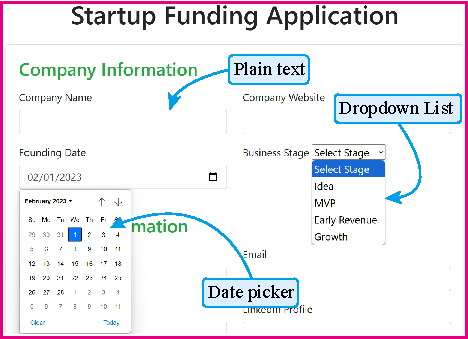
\includegraphics[width=0.78\linewidth]{figs/fig2.pdf}
    \caption{Example interface for a form filling task, using a startup funding application as a case study. The form contains diverse field types, including plain text inputs (e.g., company name), a date picker (e.g., founding date), and a dropdown list (e.g., business stage), illustrating the multimodal and semantically grounded nature of real-world form understanding and completion.}
    \label{fig:fig2}
\end{figure}


% \subsection{Multimodal Large Language Model}
% \label{ssec:mllm}
% Multimodal Large Language Models (MLLMs) have emerged as a transformative paradigm in AI, building upon the success of unimodal LLMs by integrating visual understanding with language reasoning. 
% Early works like CLIP~\cite{radford2021learning} and Flamingo~\cite{alayrac2022flamingo} demonstrated the potential of aligning visual and textual representations through contrastive learning and cross-attention mechanisms.
% The introduction of GPT-4V~\cite{gpt4technicalreport} marked a significant milestone, showcasing remarkable capabilities in complex multimodal tasks through proprietary architecture.
% Open-source initiatives such as BLIP-2~\cite{li2023blip2} and LLaVA~\cite{liu2023visual} established effective paradigms for combining frozen vision encoders with LLMs via learnable adapters, enabling instruction-following capabilities through curated datasets like LLaVA-Instruct.

% Recent advances have focused on scaling input resolution~\cite{liu2023improved}, supporting regional understanding~\cite{chen2023shikra}, and extending modality coverage to video~\cite{li2023videochat} and 3D data~\cite{hong2023llama}.
% Training strategies typically involve three stages: (1) vision-language alignment using web-scale datasets like LAION-5B~\cite{schuhmann2022laion}, (2) instruction tuning with GPT-4 synthesized data~\cite{liu2023visual}, and (3) human preference alignment via RLHF~\cite{fu2023mme}.
% Benchmark studies reveal persistent challenges including hallucination mitigation~\cite{yin2023woodpecker} and compositional reasoning~\cite{lu2023scienceqa}.
% Emerging architectures like Qwen-VL~\cite{bai2023qwen} and NExT-GPT~\cite{wu2023nextgpt} further push the boundaries by supporting multimodal inputs/outputs and tool integration.
% The field continues to evolve rapidly, with applications spanning medical imaging~\cite{li2023llava} and embodied AI~\cite{yang2023mmreact}.





\begin{figure*}[t]
    \centering
    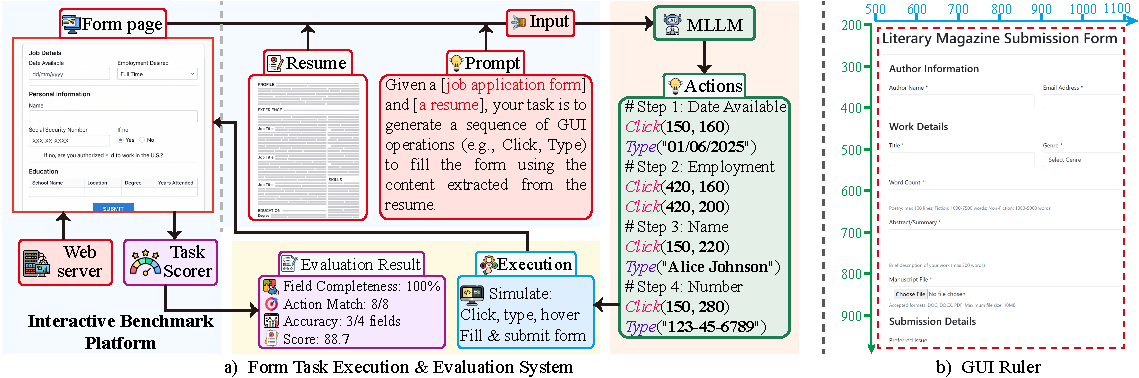
\includegraphics[width=0.98\linewidth]{figs/overview.pdf}
    \caption{
    Overview of the form-filling task system. (a) The platform takes a form and a resume as input, prompting an MLLM to generate GUI actions (Click, Type) for form completion. Execution and scoring modules evaluate task performance. (b) GUI Ruler offers pixel-level reference for visual field alignment.}
    \label{fig:system}
\end{figure*}

\section{FormFactory Benchmark}



\subsection{Platform Development}
Evaluating agents on the form-filling task using real-world platforms is often impractical.
Most existing systems are tightly coupled with proprietary interfaces, lack standardized annotations, and are not designed for large-scale or automated testing, making controlled and reproducible evaluation challenging.

To overcome these limitations, we developed a dedicated simulation platform using Python and Flask.
The platform enables interactive form-filling through standard web browsers and supports automatic backend scoring based on ground-truth key-value annotations.
It is lightweight, extensible, and suitable for evaluating both human users and multimodal agents in a controlled environment.

Our benchmark covers 20 realistic forms across 8 domains, such as academia, finance, healthcare, and IT.
Each form integrates multiple field types—including text inputs, dropdowns, date pickers, checkboxes, file uploads, and numeric fields—reflecting the multimodal and compositional challenges of the task.
As illustrated in \cref{fig:fig2}, a single form may require agents to align semantics, interpret layouts, and interact across input modalities.

In addition to field diversity, we introduce stylistic variability through changes in layout, typography, and color schemes.
The platform also supports multi-page forms and modular field definitions, enabling easy expansion to new scenarios.
These design choices ensure robustness and prevent agents from overfitting to specific templates.

Overall, our platform offers a high-fidelity, flexible, and automated environment for benchmarking form-filling agents, bridging the gap between synthetic evaluation and real-world complexity.



% \subsection{Dataset Collection}
% Our dataset comprises input documents and corresponding answers represented as key-value pairs.
% The provided inputs simulate known information typically used by humans when filling out forms.
% For instance, when submitting journal papers, substantial information (such as title, author, abstract, and keywords) is already contained within the manuscript document, allowing direct copying during form filling.
% Similarly, in job application scenarios, essential personal information such as education history commonly resides within PDF resumes.
% Conversely, in leave request scenarios, relevant details (such as leave date and location) generally originate from human memory; thus, in simulations, we provide descriptive text to mimic human verbalizations of the necessary information.
% Accordingly, our dataset includes two types of input data: textual descriptions and document-based materials.
% For each distinct type of form, we constructed 50 unique data instances through a combination of real-world and synthetic data methods.
% For the submission-related PDF documents, we utilized real-world data, acquiring 50 actual academic papers and manually annotating key information to extract corresponding key-value pairs.
% For other form types, we adopted a synthetic data generation approach.
% Specifically, our synthetic data construction process consists of two main steps:
% Initially, given a specific form and its fields, we prompt a large language model (LLM) to generate diverse key-value pairs containing randomized information.
% Subsequently, based on these key-value pairs, we instruct the LLM to produce coherent descriptive paragraphs containing the specified information.
% For static fields, we mandate strict adherence to the original key-value pairs, whereas for more flexible fields (e.g., personal statements), slight variations are permissible.
% Through this methodology, we generated a total of 1,250 data instances; detailed statistical results are illustrated in \cref{tab:form_stats}.


\subsection{Dataset Collection}

We construct a dataset of input documents paired with key-value annotations, simulating the types of information typically referenced by humans when completing forms. Inputs include either document-based materials (e.g., resumes, academic papers) or free-text descriptions (e.g., for leave requests).

For each form type, we generate 50 instances using either real or LLM-synthesized data.
Most forms, such as scholarship applications and workshop registrations, are constructed in two steps.
First, we generate gold-standard field values directly from the form schema.
Then, we prompt an LLM to produce a natural language description that implicitly contains these values, simulating the type of input a human user might provide.
The generated description serves as the model’s input, while the predefined field-value pairs are used as supervision targets.
% Most forms, such as scholarship applications and workshop registrations, are created by first generating field values based on the form schema and then prompting an LLM to produce natural language descriptions that embed these values.
Job application forms follow a similar process, where the LLM is instructed to generate 50 detailed Markdown-style resumes containing rich personal and professional information.
For academic submission forms, we collect 50 real papers from the web and extract structured metadata—such as title, authors, and abstract—as ground truth annotations.

As shown in \cref{tab:form_stats}, this process yields a high-quality dataset of 1,250 instances spanning diverse scenarios. In total, the dataset includes 13,800 annotated field-value pairs across various field types. In addition to basic string inputs, it covers more complex types such as date pickers, dropdowns, checkboxes, multi-select options, and numerical inputs—requiring both textual understanding and layout-aware reasoning, thus posing a significant challenge to current models.



% \begin{figure*}[htbp]
%   \centering
%   \begin{adjustbox}{max width=\textwidth}
%     \begin{subfigure}{\widthof{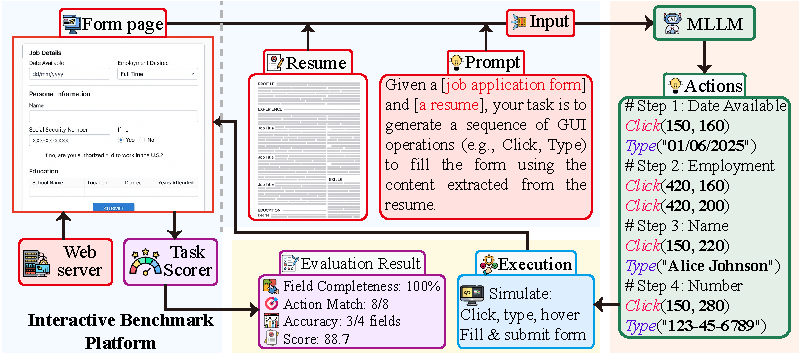
\includegraphics{figs/systemoverview.pdf}}}
%       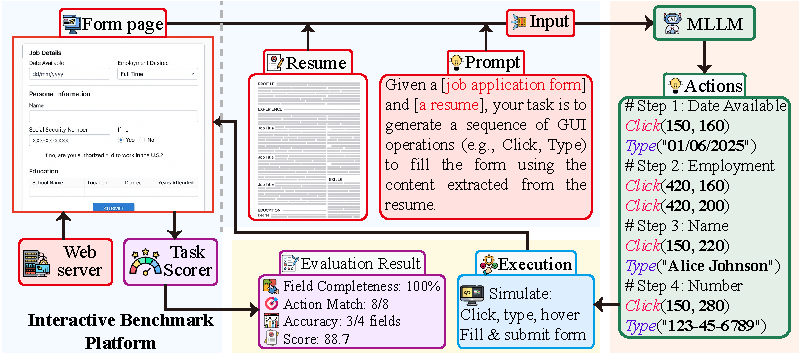
\includegraphics[height=4cm]{figs/systemoverview.pdf}
%       \caption{Caption for Figure 1}
%     \end{subfigure}
%     \hspace{1em}
%     \begin{subfigure}{\widthof{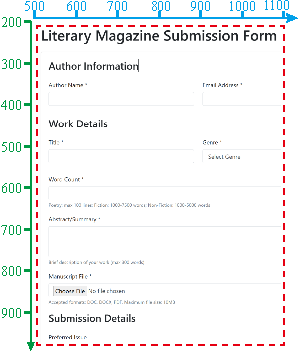
\includegraphics{figs/ruler.pdf}}}
%       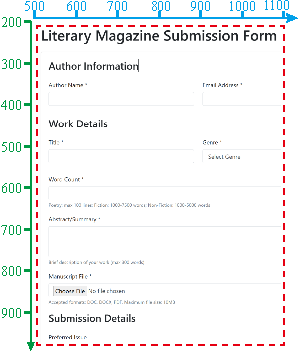
\includegraphics[height=4cm]{figs/ruler.pdf}
%       \caption{Caption for Figure 2}
%     \end{subfigure}
%   \end{adjustbox}
%   \caption{Main caption describing both figures.}
% \end{figure*}

% \subsection{Task Definition}

% We define the form-filling task as a page-level sequential decision process $(c, \mathcal{E}, \mathcal{S}, \mathcal{A})$, where:

% $c$ is the user-provided input (e.g., a resume or descriptive paragraph),

% $\mathcal{E}$ is the interactive web-based form environment,

% $\mathcal{S}$ is the state space consisting of visual observations,

% $\mathcal{A}$ is a flat set of atomic GUI actions.

% At each step $t$, the agent observes the current page $s_t \in \mathcal{S}$ and outputs a sequence of actions $\mathbf{a}_t = {a_t^1, a_t^2, \dots, a_t^k}$ to interact with the form. These actions aim to complete as many fields on the current page as possible. The agent then triggers a page-turning action (e.g., \texttt{Click(Next)}), and the process repeats until final submission.

% The observation $s_t$ is a screenshot of the current viewport. The input $c$ contains the semantic content required to complete the form, which the agent must extract, align with field labels, and translate into executable operations.

% % The action space $\mathcal{A}$ includes only two atomic operations:
% % \begin{itemize}
% % \item \texttt{Click(x, y)} — mouse click at pixel coordinates $(x, y)$;
% % \item \texttt{Type(text)} — type a string into a focused input field.
% % \end{itemize}
% The action space $\mathcal{A}$ is primarily composed of two atomic operations:
% \begin{itemize}
% \item \texttt{Click(x, y)} — mouse click at pixel coordinates $(x, y)$;
% \item \texttt{Type(text)} — type a string into a focused input field.
% \end{itemize}
% In addition, other low-level actions such as \texttt{RightClick}, \texttt{DoubleClick}, or \texttt{Ctrl}-key combinations may be required in specific cases (e.g., special buttons, modal triggers), though they are not the primary focus of our current benchmark.


% Higher-level behaviors—such as selecting a dropdown option, picking a date, or checking a box—are realized through combinations of these basic actions. For instance, interacting with a dropdown involves clicking to open it, then clicking again to choose an option. These interactions may trigger transient UI states (e.g., overlays or modal popups), requiring the agent to handle hierarchical operations through visual feedback.

% Our agent operates under a greedy page-wise policy, aiming to generate all applicable actions for the current page in a single decision step. This formulation reflects natural user workflows and improves efficiency by reducing unnecessary turn-level predictions.

% A reward signal can be assigned based on the correctness of the submitted form values, with partial credit given for incomplete but accurate entries. This enables both supervised and reinforcement-style training and evaluation.




\subsection{Task Definition}

We formalize the form-filling task as a page-level sequential decision process $(c, \mathcal{E}, \mathcal{S}, \mathcal{A})$, where $c$ is the user input (e.g., a resume), $\mathcal{E}$ is the interactive web environment, $\mathcal{S}$ the visual state space (screenshots), and $\mathcal{A}$ a flat set of atomic actions.

% At each step $t$, the agent receives the user context $c$ and observes the current visual state$s_t \in \mathcal{S}$ and outputs a sequence of actions $\mathbf{a}_t = {a_t^1, a_t^2, \dots, a_t^k}$ to complete fields on the current page. Once done, it triggers a page-turning action (e.g., \texttt{Click(Next)}), repeating the process until submission.
% At each time step $t$, the agent receives the user context $c$ and observes the current visual state $s_t \in \mathcal{S}$ (i.e., a screenshot of the current page). Based on $(c, s_t)$, it selects a sequence of executable actions $\mathbf{a}_t = {a_t^1, a_t^2, \dots, a_t^k}$ to interact with the form (e.g., typing values or clicking elements). When all relevant fields on the current page are filled, the agent performs oa page-turning action (e.g., \texttt{Click(Next)}), and proceeds to the next page, repeating the process until final submission.
At each step $t$, the agent observes the user input $c$ and current state $s_t \in \mathcal{S}$, then outputs a sequence of actions $\mathbf{a}_t = {a_t^1, a_t^2, \dots, a_t^k}$ to complete fields on the current page. Once done, it triggers a page-turning action (e.g., \texttt{Click(Next)}), repeating the process until submission.
The action space primarily includes:
\begin{itemize}
\item \texttt{Click(x, y)} — mouse click at pixel coordinates;
\item \texttt{Type(text)} — text input into a focused field.
\end{itemize}
% Other low-level actions (e.g., \texttt{DoubleClick}, \texttt{RightClick}) may be needed occasionally but are not the focus of this benchmark.
Other low-level actions (e.g., \texttt{DoubleClick}, \texttt{RightClick}) may also be involved in our benchmark, but they are relatively rare.

Complex interactions (e.g., dropdowns, checkboxes, date pickers) are composed of basic actions. Our agent adopts a greedy page-wise policy, generating all applicable actions in one pass per page to reflect natural user workflows and improve efficiency.

\section{Methods}

\begin{table*}[!t]
\rowcolors{3}{gray!15}{white}
\setlength{\abovecaptionskip}{0.15cm}
\setlength{\belowcaptionskip}{0cm}
\centering
\resizebox{0.97\textwidth}{!}{%
  \begin{tabular}{l cc cc cc cc cc cc cc cc cc}
    \toprule
    \multirow{2}{*}{\textbf{Model}}
      & \multicolumn{2}{c}{\textbf{String}}
      & \multicolumn{2}{c}{\textbf{Drop-down List}}
      & \multicolumn{2}{c}{\textbf{Checkbox}}
      & \multicolumn{2}{c}{\textbf{Radio Button}}
      & \multicolumn{2}{c}{\textbf{Description}}
      & \multicolumn{2}{c}{\textbf{Date}}
      & \multicolumn{2}{c}{\textbf{Check}}
      & \multicolumn{2}{c}{\textbf{Episodic}} \\
    \cmidrule(lr){2-3} \cmidrule(lr){4-5} \cmidrule(lr){6-7} \cmidrule(lr){8-9}
    \cmidrule(lr){10-11} \cmidrule(lr){12-13} \cmidrule(lr){14-15} \cmidrule(lr){16-17}
        & \textbf{Click} & \textbf{Value}
      & \textbf{Click} & \textbf{Value}
      & \textbf{Click} & \textbf{Value}
      & \textbf{Click} & \textbf{Value}
      & \textbf{Click} & \textbf{Value}
      & \textbf{Click} & \textbf{Value}
      & \textbf{Click} & \textbf{Value}
      & \textbf{Click} & \textbf{Value} \\
      % & \textbf{Clk.} & \textbf{Val.}
      % & \textbf{Clk.} & \textbf{Val.}
      % & \textbf{Clk.} & \textbf{Val.}
      % & \textbf{Clk.} & \textbf{Val.}
      % & \textbf{Clk.} & \textbf{Val.}
      % & \textbf{Clk.} & \textbf{Val.}
      % & \textbf{Clk.} & \textbf{Val.}
      % & \textbf{Clk.} & \textbf{Val.} \\
    \midrule
    GPT 4o               & 2.2 & 17.5 & 0.0 & 30.7 & 0.0 & 31.3 & 0.0 & 10.0 & 8.8 & 0.8407 & 0.0 & 2.8  & 0.0 & 9.8  & 0.9 & 11.3 \\
    Gemini 2.5 Pro       & 0.9 & 98.7 & 0.0 & 99.0 & 0.0 & 76.1 & 0.0 & 52.6 & 8.1 & 0.7195 & 0.0 & 99.7 & 0.0 & 79.8 & 0.4 & 70.7 \\
    Claude 3.7 Sonnet    & 0.0 & 95.2 & 0.0 & 66.2 & 0.0 & 72.0 & 0.0 & 97.9 & 0.0 & 0.6989 & 0.0 & 99.1 & 0.0 & 55.7 & 0.0 & 58.0 \\
    Qwen-VL-Max          & 4.6 & 97.1 & 1.7 & 98.9 & 0.0 & 91.8 & 0.0 & 99.0 & 11.1 & 0.7386 & 0.0 & 98.6 & 0.0 & 71.4 & 1.1 & 72.7 \\
    Grok 3               & 0.0 & 96.2 & 0.0 & 91.2 & 0.0 & 92.4 & 0.0 & 98.1 & 5.9 & 0.7137 & 0.0 & 97.9 & 0.0 & 75.5 & 0.0 & 70.7 \\
    Doubao-vision-pro-32k & 0.0 & 94.2 & 0.0 & 89.7 & 0.0 & 38.6 & 0.0 & 96.9 & 0.0 & 0.5094 & 0.0 & 92.1 & 0.0 & 69.9 & 0.0 & 64.7 \\
    \bottomrule
  \end{tabular}%
}
\caption{
Atomic-level and episodic-level evaluation of MLLMs across different field types using Clk. and Val. metrics. GPT-4o often refuses execution despite strong capabilities, resulting in lower atomic scores. The relatively high Clk. accuracy on \textbf{Description} fields stems from their large input area, which tolerates less precise clicks. Episodic results measure end-to-end form completion accuracy.
}
\label{tab:combined}
\vspace{-10pt}
\end{table*}
% \vspace{-10pt}


\subsection{LLM-Driven Form Filling}
To enable automated execution and evaluation of form-filling tasks, we develop a lightweight MLLM-driven framework, as illustrated in \cref{fig:system} (a). The interactive benchmark system consists of three key components: a web-based form frontend, a backend task scorer, and an agent execution module.

% Given a form page and an associated input document (e.g., a resume), the LLM receives a prompt instructing it to generate a sequence of GUI-level actions—such as Click(x, y) and Type(text)—to populate the form based on the extracted content. These actions are then programmatically executed on the web interface using automation tools (e.g., PyAutoGUI\footnote{\url{https://pyautogui.readthedocs.io/en/latest/}}).
Given a form page and an associated input document (e.g., a resume), the LLM receives a prompt instructing it to generate a sequence of GUI-level actions—such as Click(x, y) and Type(text)—to populate the form based on the extracted content. These actions are then programmatically executed on the web interface using automation tools (e.g., PyAutoGUI \cite{pyautogui}).

Once the form is submitted, the backend scorer compares the generated entries against ground-truth key-value annotations and produces a detailed evaluation report, including field-level accuracy, action match rate, and an overall task score. This framework supports scalable, fine-grained analysis of model behavior in realistic form-filling scenarios.

% We first present the overall design of our form-filing task execution \& evaluation system .
% As illustrated in the figure, our evaluation suite consists of three primary components: a web interface, a frontend dataset, and a backend evaluation system. 
% % \bobo{评测框架图(Bobo),偏系统架构}
% The web interface encompasses various forms commonly encountered in daily life, such as job applications, paper submissions, and leave requests.
% These forms contain diverse types of fields, including text fields, drop-down lists, and checkboxes.
% The frontend dataset consists of either file-based or textual document descriptions, as well as field-related key-value pairs; for example, a PDF résumé paired with corresponding key-value fields from a job application website.
% The evaluation backend primarily functions to receive interactive results from the web interface and subsequently analyzes accuracy by comparing the submitted model outputs with the ground truth data.
% Specifically, the evaluation procedure is as follows: once the system initiates, an agent is provided with a data instance consisting of a document and associated key-value pairs.
% The agent processes the document, interprets the data, and subsequently begins populating the relevant form.
% Through visual perception of screen content, the agent incrementally completes each field with corresponding values by generating mouse and keyboard operations.
% Upon completion, the agent clicks the submit button; the evaluation backend receives the submitted data and retrieves the standard answers from a database.
% Performance evaluation is conducted by comparing the annotated standard answers against the model-submitted data.

% \subsection{Interactive Platform}
% Currently, several platforms exist for evaluating GUI-based agents, generally categorized into two paradigms: screenshot-based and interactive approaches.
% The advantage of the screenshot-based approach lies in its convenience and standardized format; however, it is relatively inflexible.
% Specifically, for multi-step operations, screenshot-based data typically record only a single true click path, which significantly constrains other possible interaction routes—meaning an error at one step leads inexorably to further inaccuracies.
% Thus, the screenshot-based method exhibits limited practical utility in realistic scenarios.
% In contrast, the interactive platform employs a simulation-based approach, realistically modeling common user interfaces of popular applications and enabling agents to interact via authentic clicking and typing operations, thereby providing a more robust testing environment for GUI agents.
% Evidently, the interactive paradigm offers greater alignment with realistic scenarios and inherently supports error tolerance; nevertheless, its primary drawback lies in higher development costs.
% Given the specific objectives of our task—developing general-purpose form-filling agents capable of adaptation to diverse platforms—constructing an interactive platform is an inevitable choice.
% Moreover, our targeted form-filling scenarios typically involve single-step data entry tasks completed on a single interface, naturally aligning with the strengths of interactive platforms.
% Based on these considerations, we have locally developed an integrated interactive platform.
% Our unified platform integrates multiple forms and supports real-time clicking interactions.

% \usepackage{makecell, multiroggjw, booktabs}
% \usepackage{makecell, multirow, booktabs}
% \usepackage{pifont} % for ✓

% \section{FormFactory Benchmark}
% \subsection{Task Definition}


% \subsection{Automation Framework}
% \bobo{模型工作流;图片+文字描述 (bobo)}

\subsection{Ruler-Enhanced Strategy}

While modern Multimodal LLMs exhibit impressive reasoning capabilities, they are not trained to predict pixel-level positions with precision. Directly generating absolute coordinates for GUI actions—such as clicks on form fields—can therefore be highly unreliable.
To address this limitation, we introduce a simple yet effective Ruler-Enhanced Strategy. As shown in \cref{fig:system} (b), we overlay ruler-like axes along the horizontal and vertical edges of the form screenshot. These pixel-scale markers serve as visual references that the model can use to better infer spatial relationships and generate more accurate action coordinates.

The overall task formulation and input-output format remain unchanged. We simply augment the image input with reference scales and instruct the model to utilize them when predicting Click(x, y) operations. This lightweight intervention provides auxiliary geometric context to support spatial alignment and improve the robustness of visual grounding in form-filling tasks.

% Humans are able to click accurately on a screen primarily because they can move the mouse and use its position as a reference. In contrast, it is inherently challenging for an agent to directly predict precise click coordinates without any form of guidance—a task that even humans would find difficult without visual references. 

% To address this, we equip the agent with auxiliary tools to enhance its spatial localization capabilities. Specifically, we adopt a Ruler-Enhanced Strategy, wherein rulers are added to the sides of the screen. The agent is explicitly informed that it can utilize these rulers as spatial references to improve the accuracy of its target localization.

% \bobo{图片(Bobo)+文字描述(yuheng)}

%为什么人类可以在屏幕上点击很准确?因为人类可以移动鼠标作为参考。因此,直接让 Agent 给出点击的坐标还是很有有难度的,这一点人类也无法完成。所以,我们决定给 Agent 提供工具来让它能够更准确地进行定位:我们采用的是 Ruler-EnhancedStrategy,即在屏幕的两侧加上 Ruler,并告诉模型,它可以利用 Ruler 来参考给出定位

\section{Experiments}
\subsection{Settings}




\subsubsection{MLLM List}
We evaluate several state-of-the-art MLLMs through their public APIs, without task-specific tuning. Each model interacts with our benchmark via an automated browser interface implemented on a Windows platform using PyAutoGUI.

Given the novelty and complexity of form-filling tasks, this evaluation setting allows us to assess the models’ inherent capabilities in visual grounding, spatial reasoning, and field-value alignment—without the confounding influence of additional training or domain adaptation.
The evaluated models include GPT-4o~\cite{openai2024gpt4ocard}, Gemini 2.5 Pro~\cite{gemini}, Claude Sonnet 3.7~\cite{claude3sonnet}, Qwen-VL-Max~\cite{qwenvlmax}, Grok 3~\cite{grok32024}, and Doubao-Vision-Pro-32k~\cite{doubao}.


% % \subsubsection{MLLM List}
% % \bobo{放不下了,只介绍模型名字+引用吧 (yuheng)}

% We conducted experiments on several advanced MLLMs, including:
% \begin{itemize}
%     \item GPT-4o\cite{openai2024gpt4ocard}: OpenAI’s native MLLM with strong and balanced capabilities across text, vision, and audio.
%     \item Gemini 2.5 Pro Experimental 0325\cite{gemini}: Google DeepMind's MLLM, optimized for complex vision-language reasoning.
%     \item Claude Sonnet 3.7\cite{claude3sonnet}: Anthropic’s efficient MLLM, designed for safe and aligned vision-text understanding.
%     \item Qwen-VL-Max\cite{qwenvlmax}: An opeon-source MLLM from Alibaba, with strong performance in both image and text comprehension.
%     \item Grok 3\cite{grok32024}: xAI’s MLLM that integrates visual reasoning with web-scale textual information.
%     \item Doubao-Vision-Pro-32k\cite{doubao}: Baidu’s long-context MLLM, capable of processing high-resolution images and extended text sequences.

% \end{itemize}

% \bobo{介绍我们论文中用到的MLLm,带上引用。一个大模型一句话吧。可以用itemize 命令(yuheng)}

\subsubsection{Evaluation Metrics}

% We adopt two evaluation levels: Atomic and Episodic. The Atomic evaluation measures performance on individual field types, including:
% \textbf{String} (free text), \textbf{Drop-down List}, \textbf{Checkbox}, \textbf{Radio Button}, \textbf{Description} (open-ended), \textbf{Date selectors}, and \textbf{Check} (binary confirmation).
% In contrast, the Episodic evaluation assesses whether the model completes an entire form correctly, reflecting its holistic reasoning and coordination ability.

% For both levels, we use two complementary metrics: Click, which checks if the correct UI element was selected, and Value, which assesses whether the content was filled in correctly. Value is measured by exact match accuracy (\textbf{Acc}), except for Description fields, which use \textbf{BLEU}~\cite{papineni-etal-2002-bleu} due to their generative nature. Click accuracy is uniformly computed with \textbf{Acc}o.
% We perform both \textit{Atomic} and \textit{Episodic} evaluations. The Atomic evaluation assesses model performance on individual form elements, including: \textbf{String} (free-text input fields), \textbf{Drop-down List} (single-choice menus), \textbf{Checkbox} (multi-select options), \textbf{Radio Button} (exclusive-choice groups), \textbf{Description} (open-ended fields such as "special requirements"), \textbf{Date} (date selectors), and \textbf{Check} (binary options like agreement confirmations). Each field type is evaluated independently to capture fine-grained interaction accuracy.

% In contrast, the Episodic evaluation adopts an end-to-end perspective, measuring whether the model can correctly complete an entire form. This holistic metric reflects the model’s ability to coordinate multiple reasoning steps in a realistic workflow.

% For both evaluation levels, we report two complementary metrics: \textbf{Click}, which measures whether the model selected the correct UI element, and \textbf{Value}, which assesses whether the correct content was filled in. Value is computed using exact match accuracy (\textbf{Acc}), except for Description fields, which are evaluated using \textbf{BLEU}~\cite{papineni-etal-2002-bleu} due to their generative nature. Click is uniformly measured using \textbf{Acc} across all field types.

We conduct both Atomic and Episodic evaluations. The Atomic evaluation tests model performance on individual field types—String, Drop-down List, Checkbox, Radio Button, Description, Date, and Check—to capture fine-grained interaction accuracy. In contrast, the Episodic evaluation measures end-to-end form completion, assessing the model’s ability to coordinate multiple reasoning steps in realistic workflows.

For both levels, we report two metrics: Click, evaluating correct UI element selection (using accuracy), and Value, evaluating content correctness. Value is measured by exact match accuracy (Acc), except for Description fields, which use BLEU~\cite{papineni-etal-2002-bleu} due to their generative nature.


% \subsubsection{evaluation metric}

% We perform both \textit{Atomic} and \textit{Episodic} evaluations for each task. Specifically, the Atomic evaluation involves assessing the model's performance on individual form elements, including: \textbf{String} (free-text input fields), \textbf{Drop-down List} (single-choice from a list), \textbf{Checkbox} (multi-choice options), \textbf{Radio Button} (single-choice among multiple), \textbf{Description} (open-ended fields such as ``special requirements''), \textbf{Date} (date selectors), and \textbf{Check} (binary options such as agreement confirmations). Each of these element types is evaluated independently to quantify fine-grained interaction accuracy. In contrast, the Episodic evaluation adopts an end-to-end setting, where we assess whether the model correctly completes the entire form for a given task. This holistic evaluation reflects the model’s ability to integrate multiple reasoning and generation components in a realistic scenario.

% For both Atomic and Episodic evaluations, we assess performance using two complementary metrics: \textbf{Click} and \textbf{Value}. The Click metric measures whether the model successfully interacted with the correct UI element (e.g., whether it correctly clicked into a text input box or selected the appropriate option). The Value metric evaluates whether the model filled in or selected the correct content. For most element types, Value is evaluated using exact match accuracy (\textbf{Acc}). The exception is Description fields, which are evaluated using the \textbf{BLEU}\cite{papineni-etal-2002-bleu} score due to their open-ended and generative nature. Click accuracy is uniformly measured using \textbf{Acc} across all components.

% \bobo{介绍评价指标,click啥意思,value啥意思,episodic啥意思 (yuheng)}

% \begin{table*}[!t]
% % Zebra striping from third row (GPT 4o)
% \rowcolors{3}{gray!15}{white}
% \setlength{\abovecaptionskip}{0.15cm}
% \setlength{\belowcaptionskip}{0cm}
% \centering
% \resizebox{1.0\textwidth}{!}{%
%   \begin{tabular}{l cc cc cc cc cc cc cc cc}
%     \toprule
%     % Multirow for Model spanning two header rows
%     \multirow{2}{*}{\textbf{Model}}
%       & \multicolumn{2}{c}{\textbf{String}}
%       & \multicolumn{2}{c}{\textbf{Drop-down List}}
%       & \multicolumn{2}{c}{\textbf{Checkbox}}
%       & \multicolumn{2}{c}{\textbf{Radio Button}}
%       & \multicolumn{2}{c}{\textbf{Description}}
%       & \multicolumn{2}{c}{\textbf{Date}}
%       & \multicolumn{2}{c}{\textbf{Check}} \\
%     % Second header row: subcolumn labels
%      \cmidrule(lr){2-3} \cmidrule(lr){4-5} \cmidrule(lr){6-7} \cmidrule(lr){8-9} \cmidrule(lr){10-11} \cmidrule(lr){12-13} \cmidrule(lr){14-15}
%       & \textbf{Click(\%)} & \textbf{Value(\%)}
%       & \textbf{Click(\%)} & \textbf{Value(\%)}
%       & \textbf{Click(\%)} & \textbf{Value(\%)}
%       & \textbf{Click(\%)} & \textbf{Value(\%)}
%       & \textbf{Click(\%)} & \textbf{Value}
%       & \textbf{Click(\%)} & \textbf{Value(\%)}
%       & \textbf{Click(\%)} & \textbf{Value(\%)} \\
%     \midrule
%      GPT 4o               & 2.2 & 17.5 & 0.0 & 30.7 & 0.0 & 31.3 & 0.0 & 10.0 & 8.8 & 0.8407 & 0.0 & 2.8  & 0.0 & 9.8 \\
%     Gemini 2.5 Pro        & 0.9 & 98.7 & 0.0 & 99.0 & 0.0 & 76.1 & 0.0 & 52.6 & 8.1 & 0.7195 & 0.0 & 99.7 & 0.0 & 79.8 \\
%     Claude 3.7 Sonnet     & 0.0 & 95.2 & 0.0 & 66.2 & 0.0 & 72.0 & 0.0 & 97.9 & 0.0 & 0.6989 & 0.0 & 99.1 & 0.0 & 55.7 \\
%     Qwen-VL-Max          & 4.6 & 97.1 & 1.7 & 98.9 & 0.0 & 91.8 & 0.0 & 99.0 & 11.1 & 0.7386 & 0.0 & 98.6 & 0.0 & 71.4 \\
%     Grok 3               & 0.0 & 96.2 & 0.0 & 91.2 & 0.0 & 92.4 & 0.0 & 98.1 & 5.9 & 0.7137 & 0.0 & 97.9 & 0.0 & 75.5 \\
%     Doubao-vision-pro-32k & 0.0 & 94.2 & 0.0 & 89.7 & 0.0 & 38.6 & 0.0 & 96.9 & 0.0 & 0.5094 & 0.0 & 92.1 & 0.0 & 69.9 \\
%     \bottomrule
%   \end{tabular}%
% }
% % \caption{
% \caption{
% Atomic-level evaluation of MLLMs across different field types using Click and Value metrics. GPT-4o often refuses execution despite strong capabilities, resulting in lower scores. The relatively high Click accuracy on \textbf{Description} fields stems from their large input area, which tolerates less precise clicks.
% }
% % }
% \label{tab:gpt4o_string}
% \end{table*}




%Description的Value是BLEU分数
% 目前MLLM虽然展现出了不错的value提取能力,但是其对空间匹配于填写还是不行
%师兄,这里的 Check 指的是:就是那种“是否同意协议”,“是否订阅”这种勾选框,师兄看看用什么名词比较好(因为文本中有时并不会明确提到这一点,考验大模型是否会自动推理然后勾上)
%遗漏的直接算错
%Episodic可能会比前面的某一列值高的原因是,并不每个表都有前面所有的列(比方说有点表就没有下拉框啊什么什么的)
%Description能点到,是因为那个框大
%GPT-4o可以完成这样的任务,但是经常会拒绝,所以导致它的准确率低
%当前的MLLM具备作为表单填写Agent的潜力,但是往往难以捕捉到所有的细节,且像素级别的定位依然是难点

%我们为什么要加ruler?公平性:人为什么可以点的准?因为人有鼠标的位置作为参考。然后ruler可以讲述为tool(Agent使用ruler作为tool)。且对不同精度的ruler,模型表现都不好。

% Future Work:这样的Agent的安全性

%为什么采用纯视觉,“第一性原则”
% \subsection{Main Result}
% \bobo{写一下{bobo}}
\subsection{Main Results}

As shown in \cref{tab:combined}, most models exhibit extremely low performance on the \textbf{Click} metric—generally below 10\% across field types—indicating substantial challenges in accurate GUI interaction.
This issue is especially pronounced for structurally complex fields like checkboxes and dropdowns, where precise visual grounding and coordinate prediction are essential.
These results underscore the difficulty of our benchmark, particularly under inference-only settings without task-specific adaptation.

On the other hand, \textbf{Value} scores are relatively high.
This is partly due to our evaluation design: we consider a field correct as long as its corresponding value appears in the model’s output, regardless of whether it was actually entered into the correct UI location.
This design focuses on evaluating the model’s semantic understanding.Note that if value scores were computed based on whether the value was actually entered into the appropriate field through interaction, they would likely be significantly lower. We plan to adopt this stricter evaluation protocol in future iterations.

% While this relaxed criterion facilitates cross-model comparison, it masks deeper issues in grounding and execution.
% Notably, performance on \textbf{Checkbox} fields remains inconsistent even under this lenient setting.

In summary, existing MLLMs still struggle to complete form-filling tasks reliably. Improving spatial reasoning and field alignment remains critical for enabling practical, GUI-driven agents in office automation scenarios.
\subsection{Ruler-Enhanced methods}

% \begin{figure}
%     \centering
%     \includegraphics[width=0.9\linewidth]{figs/1.pdf}
%     \caption{Ruler1 \bobo{压缩内容,把两张图片并排放在一个单栏上,需要柱子变窄 (yuheng)}}
%     \label{fig:enter-label}
% \end{figure}

% \begin{figure}
%     \centering
%     \includegraphics[width=0.9\linewidth]{figs/2.pdf}
%     \caption{Ruler2}
%     \label{fig:enter-label}
% \end{figure}

% \begin{figure}[htbp]
%     \centering
%     \subfigure[Ruler1]{
%         \includegraphics[width=0.45\linewidth]{figs/1.pdf}
%         \label{fig:ruler1}
%     }
%     \hspace{0.01\linewidth}
%     \subfigure[Ruler2]{
%         \includegraphics[width=0.45\linewidth]{figs/2.pdf}
%         \label{fig:ruler2}
%     }
%     \caption{Comparison between Ruler1 and Ruler2.}
%     \label{fig:ruler_comparison}
% \end{figure}
\begin{figure}[htbp]
    \centering
    \begin{minipage}{0.48\linewidth}
        \centering
        \includegraphics[width=\linewidth]{figs/1.pdf}
        \label{fig:ruler1}
    \end{minipage}
    \hspace{0.01\linewidth}
    \begin{minipage}{0.48\linewidth}
        \centering
        \includegraphics[width=\linewidth]{figs/2.pdf}
        \label{fig:ruler2}
    \end{minipage}
    \vspace{-15pt}
    \caption{
    Click accuracy with and without Ruler guidance across difficulty levels. Higher group numbers (1–5) correspond to more fields and types, indicating greater task difficulty. Group 0 reflects overall performance.
    }
    % Comparison between Ruler1 and Ruler2.}
    \label{fig:ruler_res}
\vspace{-10pt}
\end{figure}


We conduct an ablation study to assess the effectiveness of the Ruler-Enhanced strategy.
As shown in \cref{fig:ruler_res}, introducing ruler guidance generally improves click accuracy, demonstrating its utility as a lightweight visual aid. The gain is more noticeable on simple forms with fewer UI elements, where spatial references help the model better align clicks with target fields. However, the improvement is marginal on complex forms requiring multiple interactions, suggesting that ruler-based guidance alone is insufficient for handling more challenging visual reasoning.

Even with ruler support, absolute click accuracy remains low, highlighting the need for more advanced strategies to improve spatial grounding and precise GUI control in form-filling tasks.

% Through experiments on forms of varying complexity, we observe that on easy forms (i.e., those with fewer UI elements), the introduction of Ruler guidance leads to a noticeable improvement in the model’s click accuracy. However, on more complex forms that require multiple clicks, the overall task completion rate improves only marginally—or not at all.

% Notably, even on simple forms, the model’s click accuracy remains low, reaching only around 20\%. Furthermore, using Rulers with different levels of precision fails to produce any significant gains in performance.
% \bobo{简单写一下分析,草稿就行。描述现象,中文也行,我来改逻辑(yuheng)}
% \bobo{写一下分析(bobo)}
\subsection{In-depth Analysis}
% \subsubsection{Pe}
\subsubsection{Value Score under Varying Field Counts}
We further analyze model performance in terms of value score under varying field complexity. As shown in \cref{fig:value_field}, all three models exhibit a clear downward trend in Value accuracy as the number of fields increases.
This reflects a natural scalability bottleneck: forms with more fields not only increase alignment difficulty but also introduce diverse field types requiring fine-grained parsing and reasoning.
Given that real-world forms often contain a large number of heterogeneous fields, this result highlights the limitations of current MLLMs and the need for more robust handling of complex form structures.

\subsubsection{Click Accuracy under Varying Field Counts}

To complement our value-based analysis, we also examine \textbf{click accuracy} across forms of increasing field counts. As shown in \cref{fig:click_trend}, the overall trend is similar—click performance declines as field count grows, due to higher visual complexity and denser layouts.
Unlike value scoring, which applies across all field types, click accuracy is reported only for \textbf{String} and \textbf{Description} fields, as model performance on others (e.g., checkbox, dropdown) is consistently near zero. Despite this filtering, the overall click accuracy remains low across all models, underscoring the difficulty of pixel-level interaction and spatial grounding even for simple text fields.

\begin{figure}[!tbp]
    \centering
    \begin{minipage}{0.49\linewidth}
        \centering
        \includegraphics[width=\linewidth]{figs/3.pdf}
        \label{fig:ruler1}
    \end{minipage}
    \begin{minipage}{0.49\linewidth}
        \centering
        \includegraphics[width=\linewidth]{figs/4.pdf}
        \label{fig:ruler2}
    \end{minipage}
    \vspace{-20pt}
    % \caption{Comparison between Ruler1 and Ruler2.}
    % \caption{Value accuracy across varying field counts (left) and field types (right).}
    \caption{Value accuracy across varying field counts (left, smoothed with a window size of 3) and field types (right).}
    \label{fig:value_field}
\end{figure}

\begin{figure}[htbp]
    \centering
    \begin{minipage}{0.49\linewidth}
        \centering
        \includegraphics[width=\linewidth]{figs/6.pdf}
        \label{fig:ruler1}
    \end{minipage}
    \begin{minipage}{0.49\linewidth}
        \centering
        \includegraphics[width=\linewidth]{figs/5.pdf}
        \label{fig:ruler2}
    \end{minipage}
    \vspace{-20pt}
    % \caption{Comparison between Ruler1 and Ruler2.}
    % \caption{Value accuracy across varying field counts (left) and field types (right).}
    \caption{Click accuracy across varying field counts (left, smoothed with a window size of 3) and field types (right).}
    \label{fig:click_trend}
\end{figure}

\begin{figure}[htbp]
    \centering
    \begin{minipage}[t]{0.45\linewidth}
        \centering
        \includegraphics[width=\linewidth]{figs/7.pdf}
        \label{fig:ruler1}
    \end{minipage}%
    \hspace{0.01\linewidth}
    \begin{minipage}[t]{0.45\linewidth}
        \centering
        \includegraphics[width=\linewidth]{figs/8.pdf}
        \label{fig:ruler2}
    \end{minipage}
    \vspace{-20pt}
    \caption{
    % Click accuracy across varying field counts (left, smoothed with a window size of 3) and field types (right).
    Click accuracy under joint variation of field count and field types for two models.
    }
    \vspace{-10pt}
    \label{fig:3d}
\end{figure}
% \vspace{-20pt}

% \begin{figure}
%     \centering
%     \includegraphics[width=0.85\linewidth]{figs/3.pdf}
%     \caption{Analysis-1}
%     \label{fig:enter-label}
% \end{figure}

% \begin{figure}
%     \centering
%     \includegraphics[width=0.85\linewidth]{figs/4.pdf}
%     \caption{Analysis-2}
%     \label{fig:enter-label}
% \end{figure}
% \subsubsection{}
% \bobo{三个实验描述(bobo)
% 1. 随着field type的增多,效果有何变化 (图:yuheng)
% 2. 随着field num的增多,效果有何变化 (图:yuheng)
% 3. 
% }
\subsubsection{Joint Effects of Field Count and Type}
While the previous sections analyzed the effects of field count and field type independently, these two factors often co-occur in real-world scenarios and jointly contribute to task complexity.
To better understand their combined impact, we conduct a 3D analysis of model performance with both variables.
As shown in \cref{fig:3d}, performance is highest when both field count and field type are low, and lowest when both are high—indicating strong compounding effects. This trend validates our benchmark design: forms with more fields and diverse field types significantly challenge the spatial reasoning, alignment, and grounding capabilities of current MLLMs.

\section{Conclusion}
In this paper, we present \textbf{FormFactory}, the first interactive benchmarking suite tailored for multimodal form-filling agents.
Our suite consists of a lightweight web platform and a diverse, realistic dataset covering a wide range of real-world scenarios. 
The benchmark is designed to simulate practical challenges, characterized by rich field types, high field counts, and complex layout variations.
We evaluate several state-of-the-art MLLMs and GUI agents under zero-shot settings.
Despite their strong performance on traditional multimodal tasks, all models exhibit severe limitations in form-filling: click success rates fall below 10\%, and end-to-end form completion rates remain under 2\%.
These results highlight that form-filling is a substantially harder task than standard GUI interaction, demanding fine-grained grounding, alignment, and reasoning.
We hope FormFactory provides a useful foundation for studying this underexplored yet practically important task.
By offering a realistic dataset, interactive interface, and standardized evaluation framework, our benchmark enables more precise diagnosis of agent limitations and facilitates systematic progress toward reliable form-filling systems.

% \bobo{结论(bobo)}

% \section{Ethical Considerations and Privacy}
% All data in FormFactory are either synthetically generated using large language models or collected from publicly available academic papers on arXiv. To protect author privacy, we edit the PDF files by replacing email addresses with randomly generated placeholders. No personal or sensitive information is included in the released dataset.

\section{Ethical Considerations, Privacy, and Licensing}

All data in FormFactory are either synthetically generated using large language models or collected from publicly available academic papers on arXiv.
To protect author privacy, we replace all email addresses in the PDF files with randomly generated placeholders.
No personal or sensitive information is included in the released dataset.
The benchmark is released under the MIT License.


% \begin{acks}
% To Robert, for the bagels and explaining CMYK and color spaces.
% \end{acks}

\bibliographystyle{ACM-Reference-Format}
\bibliography{new}

\end{document}